\documentclass[H:\workspace\担保人财务信息2\杭州大运河\HangZhouText.tex]{subfiles}
\begin{document}
\section{公司基本信息} 
\setlength{\tabcolsep}{0.35em} % for the horizontal padding
{\renewcommand{\arraystretch}{0.5} % for the vertical padding 
    \begin{longtable}{
        | p{2.2cm}
        | p{4.4cm}
        | p{2.2cm}
        | p{4.4cm}
        |}
        \caption{公司的基本信息}\\

        \toprule
        \endfirsthead

        \midrule
        \endhead 

        \bottomrule 
        \endlastfoot

        企业名称 & \multicolumn{3}{c|}{杭州市运河综合保护开发建设集团有限责任公司} \\
        \midrule
        注册地址 & \multicolumn{3}{c|}{浙江省杭州市江干区天城路85号} \\
        \midrule 
        注册编号 & 91330100749468780B & 成立日期 & 2003-12-19 \\
        \midrule 
        注册资本 & 500亿 & 实收资本 & 500亿 \\
        \midrule 
        公司性质 & 其他有限责任公司 & 所处行业 & 土木工程建筑业\\
        \midrule 
        营业范围 & \multicolumn{3}{p{11cm}|}{服务:京杭运河(杭州段)及两岸工程建设、开发、经营、管理。 
        服务:国内广告的设计、制作、代理、技术咨询与成果转让。} \\
        \midrule 
        股权结构 & \multicolumn{3}{p{11cm}|}{公司股权结构图如下: 
        \centering
        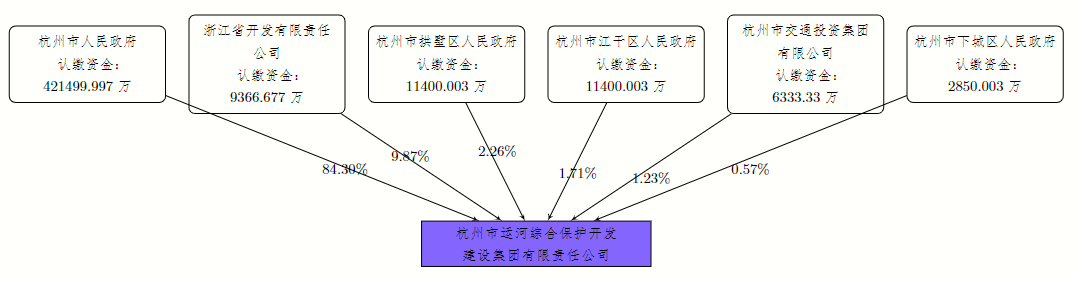
\includegraphics[width=0.72\textwidth]{img7.png}} \\
        \midrule 
        控股子公司 & \multicolumn{3}{p{11cm}|}{
        截至目前共有15家一级控股子公司(2021年12月17日天眼查查询),明细如下(单位:万元):
        \centering 
        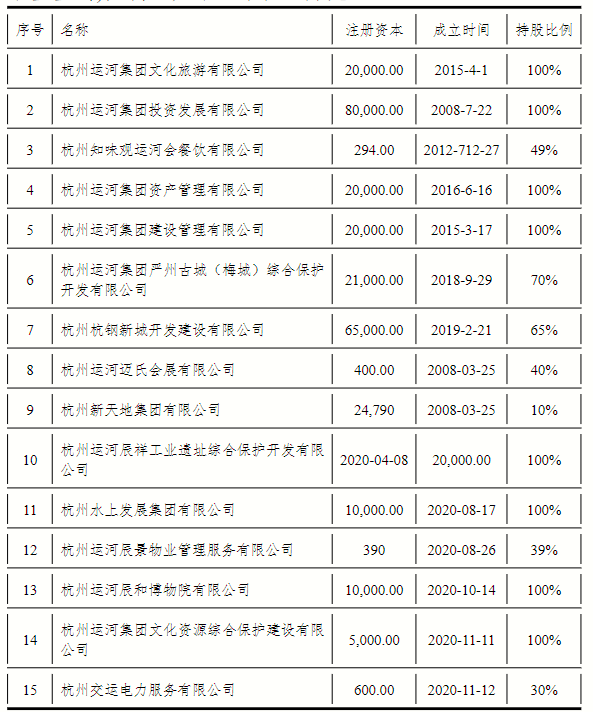
\includegraphics[width=0.5\textwidth]{img6.png}} \\
    \end{longtable}
}

\newpage 
\section{与运河相关的业务}
公司作为京杭运河杭州段综合保护开发和建设运营主体,具体负责京杭运河杭州主城区段沿岸的土地开发利用、
公共配套设施建设、项目建设和运营管理,建设重点是城中村改造、污染企业搬迁和运河水环境治理。
同时,开展资本运作和资产经营活动,重点发展以旅游休闲、文化创意产业为主的现代服务业。
2018 年末公司开发范围进一步拓展至大城北区域-杭钢新城,2020 年以来继续承担京杭运河杭州段沿岸的重
大基础设施及配套项目建设任务。\par 
公司的主营业务由四部分构成,主要是土地开发、租赁\footnote{租赁物主要是码头、地产、公园。}、酒店营收与不动产
销售,等等。其中,土地开发收入占营收的一半以上。
\begin{table}[H]
    \xiaowuhao 
    \centering
    \setlength{\tabcolsep}{1.2em} % for the horizontal padding
    {\renewcommand{\arraystretch}{0.5} % for the vertical padding 
        \begin{tabular}{@{}ccccccccc@{}}
            \toprule 
            & \multicolumn{2}{c}{2018 年} & 
            \multicolumn{2}{c}{2019年} & \multicolumn{2}{c}{2020年} & 
            \multicolumn{2}{c}{\xiaowuhao 2021年6月} \\ 
            \cmidrule(lr){2-3} \cmidrule(lr){4-5} \cmidrule(lr){6-7} \cmidrule(lr){8-9}
            & 收入 & 毛利率 &  收入 & 毛利率 
            & 收入 & 毛利率 & 收入 & 毛利率 \\
            \midrule
            营业收入 & 15.71 & 70.29\% & 34.83 & 6.14\% & 21.26 & 55.12\% & 34.42 & 23.24\% \\
            土地开发 & 13.27 & 72.59\% & 32.06 & 34.65\% & 17.19 & 52.56\% & 31.46 & 19.35\% \\
            租赁收入 & 1.63 & 70.88\% & 1.90 & 69.94\% & 3.22 & 83.93\% & 1.77 & 68.37\% \\
            酒店经营 & 0.50 & 76.49\% & 0.45 & 39.17\% & 0.35 & 23.46\% & 0.28 & 61.90\% \\
            不动产销售 & 0.02 & 100.00 & 0.00 & 100.00 & 0.01 & 100.00 & - & - \\
            \addlinespace 
            其它 & 0.29 & -49.13\% & 0.41 & -7.32\% & 0.48 & -23.83\% & 0.03 & -294.50\% \\
            \bottomrule 
        \end{tabular}
    }
    \caption{近三年主营业务收入与毛利率(单位:亿元)}
\end{table}

\subsection{土地开发}
该公司
主要负责运河主城区段及郊区段 (石祥路以北至拱墅区界)沿岸
土地开发利用、公共配套设施建设、项目建设和运营管理等 ,并参与杭州市
大城北地区的开发建设,可持续享有上述区域内 土地开发投资收益 。同时,
公司是杭州运河景区唯一运营商,综合保护的历史街区等相关资产由公司自
主经营业务开展具备区域专营优势。\par 

京杭运河杭州段南起钱塘江三堡船闸,北至杭州余杭区塘栖镇水北地区,全长约 39 公里,分为主城区段和郊区段。 
其中,主城区段南起三堡船闸,北至石祥路,长约 14 公里,流经江干、下城、拱墅三区,两岸用地横向至第一条城
市主干道,每侧平均约 500 米,规划用地面积约 21.1 平方公里,开发主体为该公司。\par 

目前运河主城区段已基本建设完成,运河及两岸的生态功能、交通功能、旅游功能和文化功能得到了极大的提升,
未来开发建设重心集中于郊区段。郊区段从石祥路至余杭区塘栖镇水北地区,长约 25 千米,流经拱墅、余杭两区,
两岸横向用地每侧控制在约 1000 米,规划用地面积约 50 平方公里。郊区段开发主体包括该公司和杭州余杭运河
综保资产管理有限公司。其中公司主要负责范围为东至拱康路, 南至石祥路,西至京杭大运河、通益路北至拱墅区界,
规划用地面积约 7.20 平方公里。\par 

目前,公司在建及拟建项目所需投资规模仍较大,未来面临较大的资本支出压力。\par 

公司主要运作模式为在政府规定范围内实施企业搬迁、城中村改造和土地整治等工作,完成土地整治后交由土地储备
中心进行出让。根据《关于京杭运河(杭州段)综合整治与保护开发问题的专题会议纪要》(杭府纪要【2004】44 号)
的规定,《京杭运河(杭州段)综合整治和保护开发战略规划》范围内的全部土地出让金及拱墅区土地出让收益上缴市的 
30\% 用于运河整治和保护开发,其中杭州市财政局将出让土地的土地出让金的 \underline{55\%} 和拱墅区土地出让收益上缴市的 
30\% 作为公司\underline{运河两岸景点建设、基础设施建设}等的专项资金直接划付公司,计入专项应付款,市财政将土地出让金剩余的 
\underline{45\%} 部分划拨至杭州市土地储备中心,由其扣除相关费用后转拨公司,作为返还土地开发补偿费确认土地开发业务收入。\par

2020 年,公司确认土地开发收入 17.19 亿元。
\begin{table}[H]
    \centering 
    \xiaowuhao
    \setlength{\tabcolsep}{1.2em} % for the horizontal padding
    {\renewcommand{\arraystretch}{0.5} % for the vertical padding 
        \begin{tabular}{@{}c|c|c|c|c @{}}
            \toprule 
            序号 & 地块名称 & 规划用途 & 土地面积 & 出让金 \\
            \midrule 
            1 & 运河新城单元 GS1004 10 地块(原 GS1201 17)& 居住/商业 & 61.20 & 9.51 \\
            2 & 运河新城 GS1001 17 地块(原 A C4 01)& 住宅 & 51.03 &17.83 \\
            3 & 运河新城单元 GS1001 15 地块(原 A C5 01 住宅)& 40.05 & 11.16 \\ 
            4 & 运河新城单元 GS1004 11 地块(原 GS1201 06)& 居住/商业 & 35.70 & 7.40 \\
            5 & 运河新城单元 GS1004 12 地块(原 GS1201 07)& 居住/商业 & 35.40 & 7.33 \\
            6 & 运河新城单元 GS1004 01 地块(原 GS1201 03)& 住宅 & 35.25 & 11.92 \\
            7 & 三里亭单元JG0906 06 地块 & 商业商务 & 8.85 & 2.12 \\
            \addlinespace
            \midrule 
            \multicolumn{3}{c|}{合计} & 267.48 & 67.27 \\
            \bottomrule 
        \end{tabular}
    }
    \caption{截至2021年3月末公司已收储未出让地块清单(单位:亿元、亩)}
\end{table}

截至 2021 年 3 月末,公司已收储未出让地块共 7 宗,土地面积合
计 267.48 亩,地块预估出让金合计为 67.27 亿元。
截至 2021 年 3 月 末,公司在开发土地开发项目主要包括运河新城地块、杭钢新城单元和三里亭地块,
总投资 272 80 亿元,已完成投资 160.95 亿元,尚需投资 111.85 亿元。
\begin{table}[H]
    \centering 
    \xiaowuhao
    \setlength{\tabcolsep}{1.2em} % for the horizontal padding
    {\renewcommand{\arraystretch}{0.5} % for the vertical padding 
    \begin{tabular}{@{}c|c|c|c|c@{}}
        \toprule 
        主要在建项目名称 & 总投资 & 已完成投资 & 面积 & 建设时间 \\
        \midrule 
        运河新城地块 & 136.37 & 74.74 & 10,797 & 2009 \textasciitilde 2023 年 \\ 
        杭钢新城单元 & 16.43 & 11.21 & 696 & 2018 \textasciitilde 2025 年 \\ 
        三里亭单元地块 & 16.43 & 11.21 & 696 & 2018 \textasciitilde 2021 年 \\
        \midrule 
        合计 & 272.80 & 160.95 & 14,173 & - \\
        \bottomrule 
    \end{tabular}
    }
    \caption{主要在建项目清单(单位:亿元,亩)}
\end{table}
 
\newpage   

\subsection{杭钢新城项目}
\subsubsection{项目建设背景}
1957年4月2日,浙江钢铁厂(杭钢的前身)开工建设,2007年,国务院批复同意《杭州市城市总体规划(2001年 \textasciitilde 2020年)》,
规划中提出"远期搬迁杭钢。2009年7月,浙江省政府发布《浙江省钢铁产业转型升级规划》,提出“积极探讨并推动杭钢与国内大
型钢铁企业集团的合作,在相关条件基本具备后,杭州厂区适时退出炼钢炼铁,重点发展钢铁冷轧及深加工,
以钢铁为重点的仓储、物流、贸易等现代服务业”。2015年12月22日,杭钢正式关闭。2017年1月,杭州市规划局组织专家对杭钢
新城编制方案进行审查,根据该方案,杭钢新城区块总计约 40,000 亩土地(26.7平方公里)。
\subsubsection{项目介绍}
\begin{wrapfigure}{l}{0.5\textwidth} % this figure will be at the left
    \centering 
    \includegraphics[width=0.4\textwidth]{img3.png}
    \caption{规划图:1}
    \label{fig:a}
\end{wrapfigure}

2018 年 9 月,根据府办简复(第 B20181614 号)公文,杭州
市政府同意公司作为大城北地区杭钢新城的土地整理及基础设施建设的主体。
根据《杭州市人民政府关于《杭州市运河新城单元(GS10)控制性详细规划(2020版)》
和《杭州市杭钢单元(GS13)控制性详细规划(2020版)》的批复》,
杭钢新城东至 320 国道,南至金昌路,西至杭宁高铁、沿山港,北至拱墅区界,规划用地面积为 565.80 万平方米。
定位为大城北核心区的东部组团,集休闲文化中心(城北副中心“东翼”)、品质居住、新兴产业等功能为一体,
以工业遗产活化利用为特色的新标志性区域。目标是打造城北转型新引擎,工业遗产新地标,城北副中心新节点。\par 

\begin{wrapfigure}{r}{0.5\textwidth}
    \centering 
    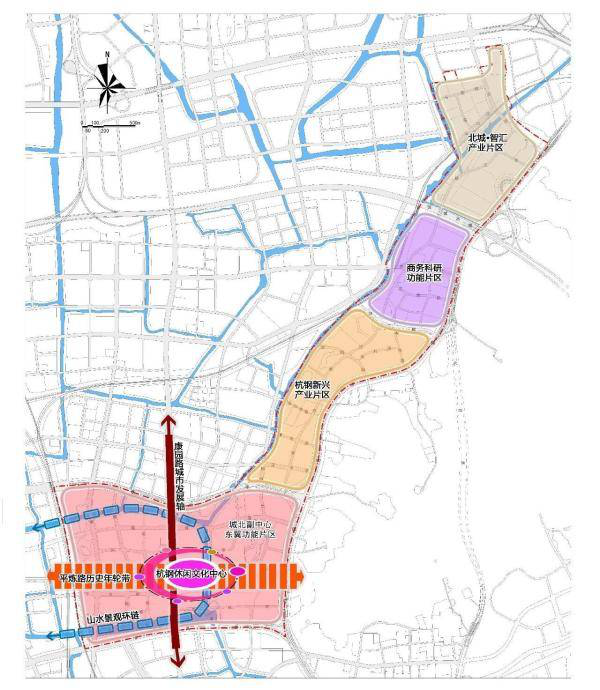
\includegraphics[width=0.5\textwidth]{img4.png}
    \caption{规划图:2}
    \vspace{-1cm}
    \label{fig:b}
\end{wrapfigure}

根据《杭钢单元规划》(以下简称《规划》),杭钢新城单元被规划形成 “一心一带、一轴一环、四片区”的功能结构,即
\begin{itemize}
    \item “一心”:即杭钢休闲文化中心,也是城北副中心的“东翼”。
    \item “一带”:即平炼路历史年轮带。
    \item “一轴”:即康园路城市发展轴。
    \item “一环”:即电厂河、吴家角港、杭钢河、大运河山水景观环链的组成部分。
    \item “四片区”:即康桥路以南的综合功能片区、康桥路以北到刘一路的杭钢新兴产业片区、
    刘一路以北至绕城高速公路的商务科研功能片区、绕城高速公路以北的北城·智汇产业片区。
\end{itemize}

\begin{wrapfigure}{l}{0.5\textwidth}
    \centering 
    \vspace{-0.5cm}
    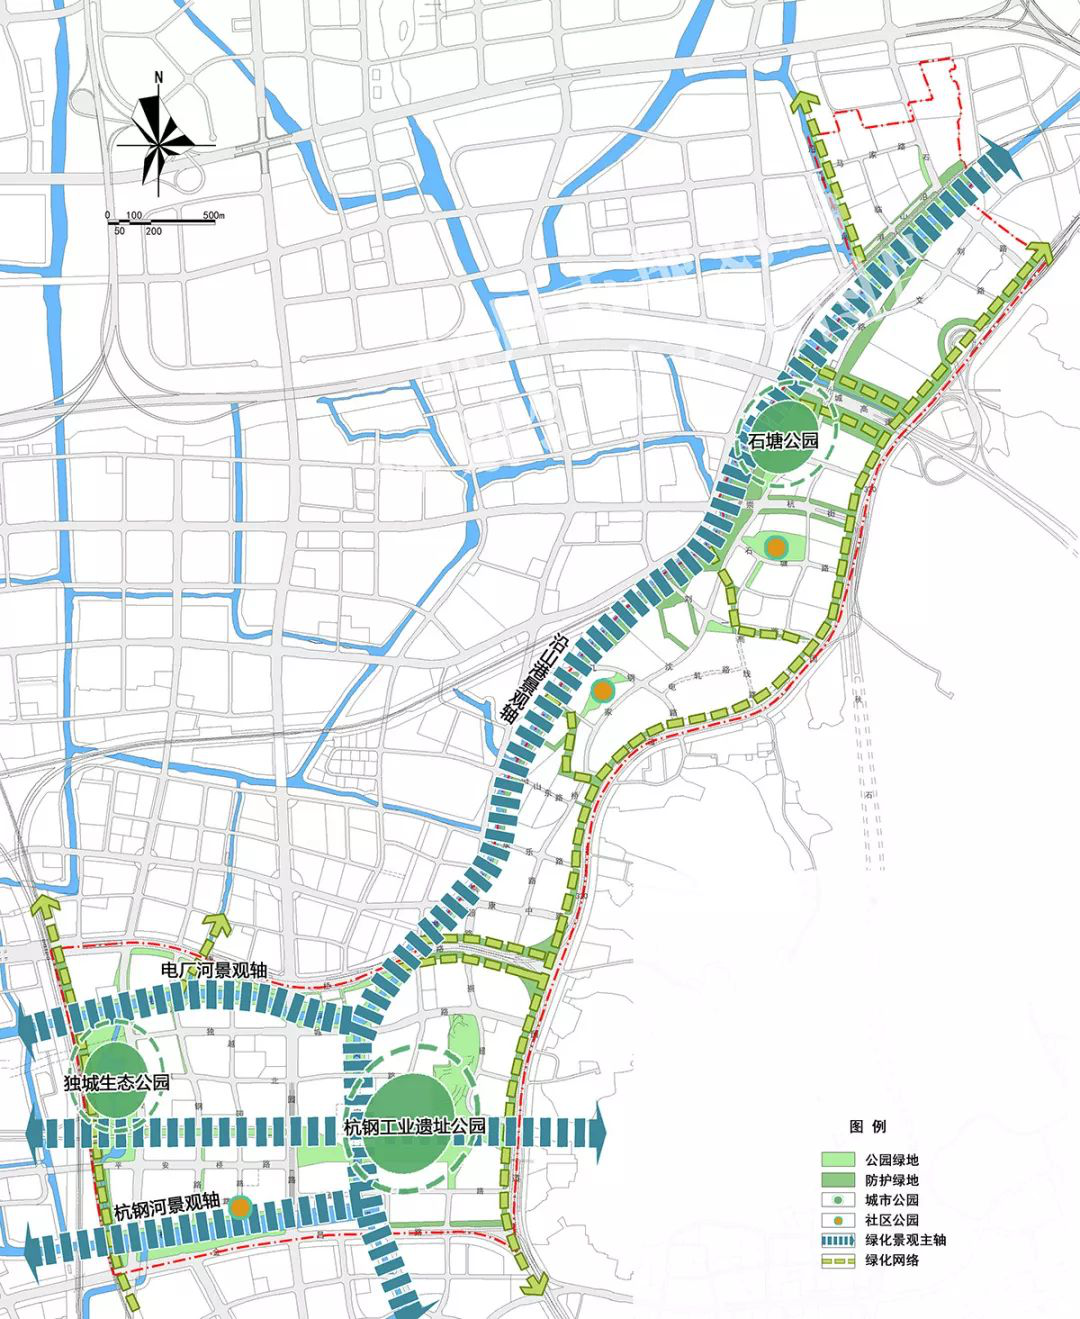
\includegraphics[width=0.4\textwidth,height=7cm]{img5.png}
    \caption{规划图:3}
    \vspace{-1cm}
    \label{fig:c}
\end{wrapfigure}

同时《规划》还提出,要形成“三园、多点,轴网相联”的绿地景观结构,即
\begin{itemize}
    \item “三园”:为杭钢工业遗址公园、独城生态公园和石塘公园。
    \item “多点”:为多处社区级公园。
    \item “轴网相联”:沿着电厂河、杭钢河、沿山港一一吴家角港两侧
    绿带及平炼路历史年轮带打造三横一纵的景观主轴,沿着其他河道绿化及路侧绿化打造绿网,
    形成轴网相联的绿化景观体系。
\end{itemize}

该项目有以下亮点。第一,合理利用杭钢工业遗存保留工业记忆,委托设计院编制杭钢工业遗存保护方案,
学习德国、宝钢、首钢的改造利用经验,保存杭钢记忆,打造文化旅游产业集聚区。第二,依托和利用半山国
家森林公园资源,拱墅区成立半山文化旅游保护开发建设指挥部,统筹规划谋划半山、杭钢、田园、桃源等地块,
同时抓好地块与大运河文化带建设紧密结合的举措,将杭钢河、下塘河、电厂河以及上塘河水上运动小镇进行水系联通。

《杭州市国民经济和社会发展第十四个五年规划和二〇三五年远景目标纲要》对大城北核
心区及示范区板块建设作了规划,在十四五期间将重点打造京
杭大运河博物院、大运河杭钢工业遗址公园、大城北中央景观大道、大运河未来艺术科
技中心、大运河滨水公共空间、运河湾国际旅游休闲综合体、大运河生态艺术岛、北景
园生态公园、武林美术馆等标杆项目,带动区域全面崛起。\par 

\subsubsection{资金来源}
运营模式方面,根据杭州市政府纪要【2004】 44 号《关
于京杭运河(杭州段)综合整治和保护开发问题的专题会议纪要》的规定,《京杭运河
(杭州段)综合整治和保护开发战略规划》范围内的全部土地出让金及拱墅区土地出让
收益上缴市的 30\% 用于运河整治和保护开发,其中杭州市财政局将出让土地的土地出让
金 55\% 部分和拱墅区土地出让收益上缴市的 30\% 作为公司运河两岸景点建设、基础设施
建设等的专项资金直接划付公司,计入“专项应付款”;市财政土地出让金剩余的 45\%
部分划拨至杭州市土地储备中心,由其与公司结算,公司将返还的土地开发补偿费确认
为土地开发收入。
\begin{table}[H]
    \xiaowuhao 
    \centering 
    \setlength{\tabcolsep}{1.2em} % for the horizontal padding
    {\renewcommand{\arraystretch}{0.5} % for the vertical padding
    \begin{tabular}{@{}l|c|c|c@{}}
        \toprule 
        & 2018 年 & 2019 年 & 2020 年 \\ 
        \midrule 
        专项应付款 & 3,173,371,453.35 & 5,558,670,672.75 & 8,669,618,268.13 \\
        运河景区公共配套设施 & 3,173,371,453.35 & 5,558,592,863.35 & 8,669,500,477.76 \\ 
        安全生产费 & -- & 77,809.40 & 117,790.37 \\
        \addlinespace 
        财政补贴 & 292,714.82 & 186,667.33 & 121,903.00 \\
        \bottomrule 
    \end{tabular}
    }
    \caption{专项应付款与财政补贴(单位:元)}
\end{table}
\footnotetext{根据杭财建【2013】165号文件,水上巴士船舶建造项目由政府补助}



除此之外,公司还有多种融资渠道,截至 2021 年 9 月末,发行人借款总额为 1,026,005.25 万元,
其中短期借款 6,100.00 万元,一年内到期的非流动负债 19,950.55 万元,长期借款 610,058.40 万元,
应付债券 389,896.30 万元。该公司分别于 2021 年 1 月 及 2021 年 4 月 发行了 10 .00 亿元 21 杭州运河 MTN001 和 10 .00 亿元 
21杭州运河 MTN002 期限均为 3 年;票面利率分别为 3.85\% 和 3.65\% 募集资金全部用于偿还公司有息债务。 
截至 2021 年 4 月末, 21 杭州运河 MTN001 及21 杭州运河 MTN002 已按约定用途分别使用了 9.44 亿元和 4.39 
亿元。

\begin{table}[H]
    \xiaowuhao 
    \centering 
    \setlength{\tabcolsep}{1.2em} % for the horizontal padding
    {\renewcommand{\arraystretch}{0.5} % for the vertical padding
    \begin{tabular}{@{}l|c|c|c|c|c|c@{}}
        \toprule 
        债项名称 & 发行金额 & 期限 & 票面利率 & 债券余额 & 发行时间 & 资金用途\\
        \midrule 
        16杭运河专项债 & 10.00 & 7年 & 3.40\% & 6.00 & 2016-10-17 & 注\footnotemark \\
        20杭州运河PPN001 & 10.00 & 3年 & 3.98\% & 10.00 & 2020-09-22 & 偿还有息债务 \\ 
        21杭州运河MTN001 & 10.00 & 3年 & 3.85\% & 10.00 & 2021-01-27 & 偿还有息债务\\
        21杭州运河MTN002 & 10.00 & 3年 & 3.65\% & 10.00 & 2021-04-13 & 偿还有息债务\\
        \midrule  
        合计 & \textbf{40.00} & -- & -- & \textbf{36.00} & -- \\
        \bottomrule 
    \end{tabular}
    }
    \caption{募集资金用途明细表(单位:亿元)}
\end{table}
\footnotetext{其中 4 亿元用于补充流动资金,剩余 6 亿元 拟全部用于运河水陆交通集散服务中心停车场、
运河绿化带(康桥路 余杭界)工程停车场、运河绿化带(石祥路 金昌路)工程停车场及杭政储出【 2007 】 84 号地块
商业办公用房及商品住宅停车场}

\begin{table}[H]
    \centering 
    \xiaowuhao 
    \setlength{\tabcolsep}{1.2em} % for the horizontal padding
    {\renewcommand{\arraystretch}{0.5} % for the vertical padding
    \begin{tabular}{@{}l|c|c|c@{}}
        \toprule 
        借款单位 & 借款金额 & 年利率 & 借款期限 \\
        \midrule 
        云南国际信托有限公司 & 0.5 & 1 年期LPR 下浮 5bp & 2020-8-14 \textasciitilde 2021-2-13 \\
        上海浦东发展银行求是支行 & 0.25 & 1 年期LPR 下浮 22.22\% & 2020-3-20 \textasciitilde 2021-3-20 \\
        上海银行杭州下沙支行 & 0.25 & 1 年期LPR & 2020-6-19 \textasciitilde 2021-6-12 \\
        中国工商银行 & 0.65 & -- & 2018-6-12 \textasciitilde 2020-12-20 \\
        杭州市土地储备交易中心 & 1.7 & -- & 2020-6-17 \textasciitilde 2023-6-15 \\
        中国民生银行湖墅支行 & 0.2 & -- & 2020-6-17 \textasciitilde 2023-6-15 \\
        中国建设银行杭州之江支行 & 0.5 & -- & 2020-8-27 \textasciitilde 2023-8-26 \\
        中国工商银行艮山支行 & 0.3 & -- & 2020-10-20 \textasciitilde 2025-10-9 \\
        \bottomrule 
    \end{tabular}
    }
    \caption{短期、长期借款明细表(单位:亿元)}
\end{table}  



\subsubsection{项目进度}
杭钢新城整体投资规模预计约 320 亿元,包括征地拆迁 120 亿元和基建投资 200 亿元,现主要进行征地拆迁,
截至 2020 年 3 月末杭钢新城累计已投资约 63 亿元 尚需投资 257 亿元。整体看,公司尚需在运河新城和杭
钢新城投资逾 500 亿元。目前关于杭钢新城的在建工程如下。  
\begin{table}[H]
    \centering 
    \xiaowuhao 
    \setlength{\tabcolsep}{1.2em} % for the horizontal padding
    {\renewcommand{\arraystretch}{0.5} % for the vertical padding\
    \begin{tabular}{@{}l|c|c|c@{}}
        \toprule 
        项目名称 & 计划总投资 & 已投资 & 计划工期 \\
        \midrule 
        大运河杭钢工业旧址综保项目GS1303-08地块文体设施 & 19.87 & 0.09 & 2020 \textasciitilde 2023 \\
        大运河杭钢工业遗址综保项目GS1303-14地块公园绿地 & 16.13 & 0.87 & 2020 \textasciitilde 2023 \\
        小河公园 & 13.07 & 0.16 & 2020 \textasciitilde 2022 \\
        杭钢河景观带(康贤路—吴家角港) & 11.83 & 0.07 & 2020 \textasciitilde 2021 \\
        丽水路(石祥路-金昌路) & 10.47 & 9.17 & 2017 \textasciitilde 2021 \\
        \midrule
        在建项目小计 & \textbf{71.37} & \textbf{10.36} & -- \\
        \midrule 
        大运河杭钢工业旧址综保项目GS1303-05地块文化设施 & 8.58 & -- & 2021 \textasciitilde 2023 \\
        大运河杭钢工业旧址综保项目GS1303-06地块文化设施 & 7.53 & -- & 2021 \textasciitilde 2023 \\
        丽水路(三里洋路-康桥路) & 7.33 & -- & 2021 \textasciitilde 2023 \\
        大运河杭钢工业旧址综保项目GS1303-12地块文化设施 & 6.44 & -- & 2021 \textasciitilde 2023 \\
        大运河杭钢工业旧址综保项目GS1303-04地块文化设施 & 6.43 & -- & 2021 \textasciitilde 2023 \\
        \midrule 
        拟建工程 & \textbf{36.31} & -- & -- \\
        \bottomrule 
    \end{tabular}
    }
    \caption{截至 2021 年 3 月末公司主要在建基础设施项目情况(单位:亿元、年)}
\end{table}

整体来说,该公司开发建设资金平衡主要依赖于区域内土地开发补偿。截至 2021 年 3 月末,公司土地开发投入余额 84.63 亿元、基础设施建设投入余额 163.46 亿元,应收杭州市土地储备
中心土地开发相关款项 6.12 亿元,杭州市财政拨付待结转的运河两岸景点建设、基础设施建设等专项资金 96.07 亿元。
同期末公司已完成整理待出让的土地约 267.48 亩,计划全部于 2021 年出让;在整理土地面积 2,000 余亩,集中于运
河新城和杭钢新城。主要地块的盈利情况如下。
\begin{table}[H]
    \centering 
    \xiaowuhao 
    \setlength{\tabcolsep}{1.2em} % for the horizontal padding
    {\renewcommand{\arraystretch}{0.5} % for the vertical padding
    \begin{tabular}{@{} p{3cm}|p{2cm}|p{2cm}|p{2cm} @{}}
        \toprule 
        项目名称 & 2018 & 2019 & 2020 \\
        \midrule 
        运河新城 & 2.25 & 3.85 & 5.55 \\
        杭钢新城 & -- & -- & 1.90 \\
        三里亭 & 0.00\footnotemark & 0.91 & 1.05 \\
        \bottomrule
    \end{tabular}
    }
    \caption{主要地块的开发明细(单位:亿元)}
\end{table}
\footnotetext{实际金额为 15,160,770.00。}
\end{document}